\documentclass[11pt,spanish,a4paper]{article}
% Versión 1.er cuat 2021 Víctor Bettachini < bettachini@df.uba.ar >

% Versión 1.er cuat 2021 Víctor Bettachini < bettachini@df.uba.ar >

\usepackage[T1]{fontenc}
\usepackage[utf8]{inputenc}

\usepackage[spanish, es-tabla]{babel}
\def\spanishoptions{argentina} % Was macht dass?
% \usepackage{babelbib}
% \selectbiblanguage{spanish}
% \addto\shorthandsspanish{\spanishdeactivate{~<>}}

\usepackage{graphicx}
\graphicspath{{./figuras/}{../LaTeX/}}
% \usepackage{float}

\usepackage[arrowdel]{physics}
\newcommand{\pvec}[1]{\vec{#1}\mkern2mu\vphantom{#1}}
% \usepackage{units}
\usepackage[separate-uncertainty=true, multi-part-units=single, locale=FR]{siunitx}
\usepackage{isotope} % $\isotope[A][Z]{X}\to\isotope[A-4][Z-2]{Y}+\isotope[4][2]{\alpha}

\usepackage{tasks}
\usepackage[inline]{enumitem}
% \usepackage{enumerate}

\usepackage{hyperref}

% \usepackage{amsmath}
% \usepackage{amstext}
\usepackage{amssymb}

\usepackage{tikz}
\usepackage{tikz-dimline}
\usetikzlibrary{calc}
% \usetikzlibrary{math}
\usetikzlibrary{arrows.meta}
\usetikzlibrary{snakes}
\usetikzlibrary{decorations}
\usetikzlibrary{decorations.pathmorphing}
\usetikzlibrary{patterns}

% \usepackage[hmargin=1cm, vmargin=1cm, includeheadfoot]{geometry}
\usepackage[hmargin=1cm,vmargin=3cm, top= 0.75cm,nohead]{geometry}
% \voffset-3.5cm
% \hoffset-3cm
% \setlength{\textwidth}{17.5cm}
% \setlength{\textheight}{27cm}

\usepackage{lastpage}
\usepackage{fancyhdr}
\pagestyle{fancyplain}
\fancyhf{}
% \fancyhead{}
\setlength\headheight{28.7pt} 
\fancyhead[LE, LO]{\textbf{Física 2} (Físicos) }
% \lhead{\textbf{Física 2} (Físicos) }
\fancyhead[RE, RO]{\href{https://df.uba.ar/es/}{$\vcenter{\hbox{\includegraphics[height=1cm]{sin_texto.pdf}}}$}}
% \rhead{$\vcenter{\hbox{\includegraphics[height=1cm]{sin_texto.jpg}}}$}
% \rhead{\includegraphics[height=1cm]{sin_texto.jpg}}
% \rhead{\textcopyright {\tt DF, FCEyN, UBA}}
\fancyfoot{\href{https://creativecommons.org/licenses/by-sa/4.0/deed.es/}{$\vcenter{\hbox{\includegraphics[height=0.4cm]{cc-by-sa.pdf}}}$} \href{https://df.uba.ar/es/}{DF, FCEyN, UBA}}
% \fancyfoot{$\vcenter{\hbox{\includegraphics[height=0.4cm]{cc-by-sa.pdf}}}$ DF, FCEyN, UBA}
% \fancyfoot{{\tiny \textcopyright DF, FCEyN, UBA}}
\fancyfoot[C]{ {\tiny Actualizado al \today} }
\fancyfoot[RO, LE]{Pág. \thepage/\pageref{LastPage}}
\renewcommand{\headrulewidth}{0pt}
\renewcommand{\footrulewidth}{0pt}


\begin{document}
\begin{center}
\textbf{Física 2} (Físicos) \hfill \textcopyright {\tt DF, FCEyN, UBA}\\
%	\textsc{\large Física 2 (Físicos)} - Prof. Diana Skigin - 2"o cuat. 2014\\
%	\textsc{\large Primer Cuatrimestre - 2014}\\
	\textsc{\LARGE Oscilador armónico de un único grado de libertad}\\
\end{center}


\begin{enumerate}

\section*{Péndulo ideal}
\item Escriba y resuelva las ecuaciones de movimiento para un péndulo de longitud $l$ en presencia de un campo gravitatorio de constante $g$. Discuta todas las aproximaciones que realiza.



\section*{Resortes antagónicos}
\item El sistema de la figura muestra un peso, de masa $m$, suspendido equidistante de dos paredes por dos resortes antagónicos de idéntica constante elástica $k$.
\begin{figure}[H]
	\centering{}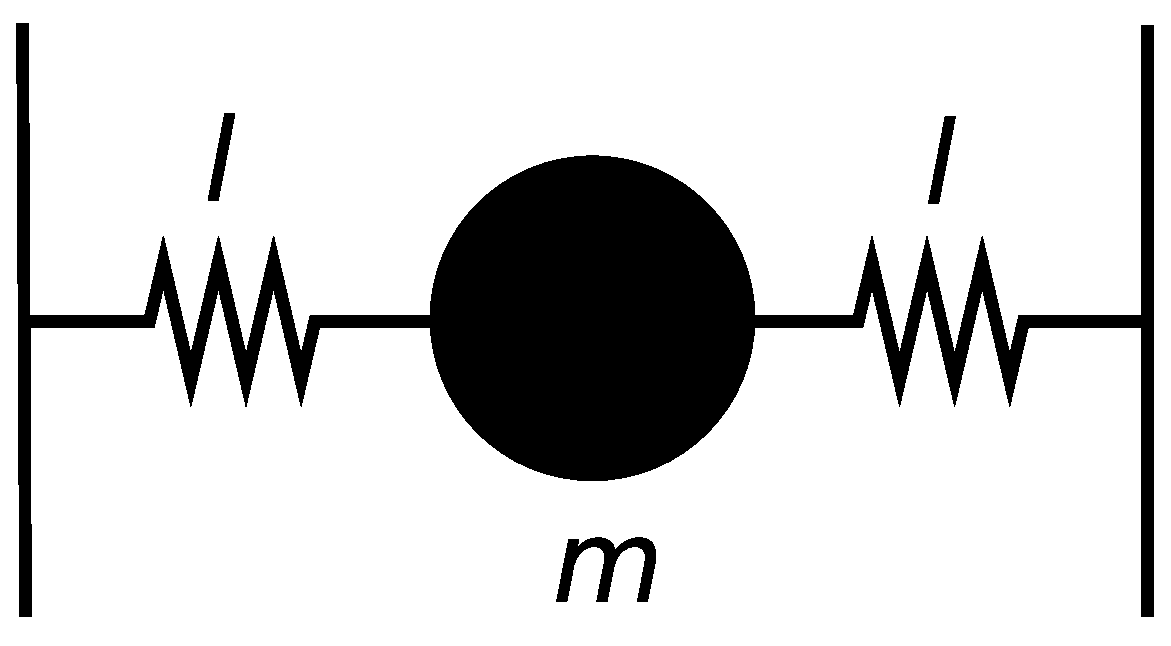
\includegraphics[clip,scale=0.25]{ej1-1}
\end{figure}
\begin{enumerate}
	\item Oscilaciones longitudinales para los casos:   
	\begin{enumerate}
		\item longitud natural del resorte $l_0$ ($l_0<l$),   
		\item ``slinky'' ($l_0=0$).   
	\end{enumerate}
	\item Oscilaciones transversales del sistema del punto anterior, discutiendo las diferencias entre los casos 1) y 2), y analizando cuidadosamente las aproximaciones que realiza.
	En el caso 1) analice la diferencia entre considerar que los resortes están tensionados en la posición de equilibrio $(l_{0}<l)$ o que están relajados en dicha posición $(l_0= l)$.
\end{enumerate}


				
\end{enumerate}

\end{document}
